% !TeX document-id = {6968f34d-f8ff-4821-863c-fafaf004332d}
% !TeX TXS-program:compile = txs:///pdflatex/[--shell-escape]
\documentclass{beamer}
\usetheme{AnnArbor}
\usefonttheme[onlymath]{serif} 
\usepackage[spanish]{babel}
\usepackage{lmodern}
\usepackage[T1]{fontenc}
\usepackage[utf8]{inputenc}
\usepackage{amsmath}
\usepackage{amsfonts}
\usepackage{amssymb}
\usepackage{graphicx}
\usepackage{epstopdf}
\usepackage{hyperref}
%\usepackage{minted}
\usepackage{adjustbox}
\usepackage{algorithm,algorithmic}


\setbeamerfont{author in head/foot}{size={\fontsize{3.5pt}{5pt}\selectfont}}
\author{Prof. Sebastian Saaibi \& David Cardozo\inst{1}}
% - Give the names in the same order as the appear in the paper.
% - Use the \inst{?} command only if the authors have different
%   affiliation.
\title{Introducción a Métodos Numéricos  }
\subtitle{Uso de Métodos Numericos, Metodos de Bracket: bisección, Metodos Abiertos: Newton - Raphson} % A subtitle is optional and this may be deleted
%\logo{\includegraphics[height=0.8cm]{universidaddelosandes.png}\vspace{220pt}} 
\logo{
\includegraphics[height=0.8cm]{universidaddelosandesciencias.png}}
%\logo{\includegraphics[height=0.8cm]{universidaddelosandescolombia.png}
\institute[Universidad de los Andes]
{
	\inst{1}%
	Física   \\
	Lectura $8$ Herramientas Computacionales \\
	Universidad de los Andes
}
\date{\today} % - Either use conference name or its abbreviation.
\subject{PDF Information} % This is only inserted into the PDF information catalog. Can be left out. 
%\setbeamercovered{transparent}
%\setbeamertemplate{navigation symbols}{}

\begin{document}
\maketitle
\begin{frame}
	\frametitle{Generalidades}
	\tableofcontents
\end{frame}


\section{Métodos Numéricos ¿Por que el énfasis?  }

\begin{frame}{fragile}
	\frametitle{Métodos Númericos}
	
	Métodos numéricos es la reunión y estudio de técnicas para resolver problemas matemáticos con operaciones aritméticas, en general requieren de \textbf{demasiadas} iteraciones de operaciones aritméticas.
	\vspace{1cm}
	Para contrastar:
	\begin{tabular}{|c|c|}
		\hline Métodos no-computacionales & "Malo" \\ 
		\hline Soluciones analíticas & La mayoría de problemas no son analíticos \\ 
		\hline Soluciones Gráficas  & No son exactas ``ojimetro'' \\ 
		\hline  Uso de calculadoras & Realizar muchas operaciones  \\ 
		\hline 
	\end{tabular}  
	
\end{frame}

\begin{frame}{fragile}
	\frametitle{Métodos Numéricos 2}
	Hagamos observaciones sobre la siguiente función: 
	\begin{figure}
		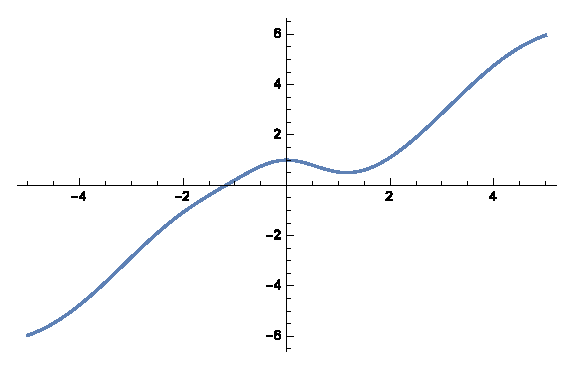
\includegraphics{Graph1}
		\caption{$ f(x) =  e^{-x^2} + x - \sin(x)$ }
	\end{figure}
	
\end{frame}

\begin{frame}{fragile}
	\frametitle{Métodos Numéricos 2}
	\begin{figure}
		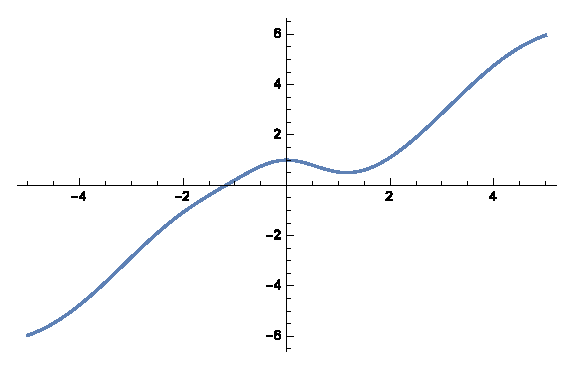
\includegraphics{Graph1}
	\end{figure}
	\[ x \approxeq -1.17426 \implies f(x) \approx 0  \]
\end{frame}


\section{Métodos de Bracket}

\begin{frame}
	\frametitle{Metodos de Bracket}
	Un poco de terminología.
	\begin{block}{Raiz}
		Dada una función $ f(x) $, en ejemplo, $ f(x) = (x+3)(x-2)^2 $ , llamamos $ x_0 $ una raiz si $ f(x_0) = 0 $
	\end{block}
	Los \textbf{métodos de bracket} aprovechan que una función cambia de signos en la vecindad de una raíz. El nombre viene porque se requieren \textbf{dos} \textbf{conjeturas o pistas}.
\end{frame}


\begin{frame}[fragile]
	\begin{figure}
		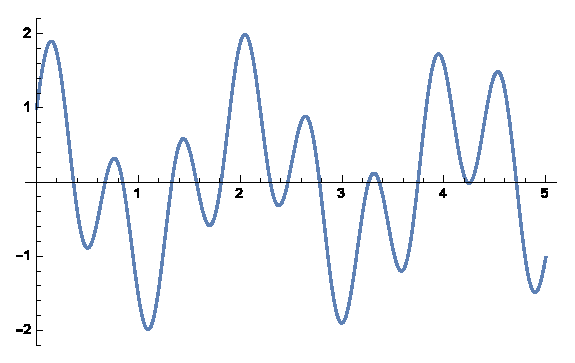
\includegraphics{Graph2}
		\caption{$ g(x) = \sin(10x) + \cos(3x) $}
	\end{figure}
\end{frame}

\subsection{Método de Bisección}

\begin{frame}
	Por el ejemplo anterior nos hemos dado cuenta que $ g(x) $ cambia de signos en lados contrarios de la raiz, es decir si $ f(x) $ es real y continuos en el intervalo $ x_{i} $ ``inferior'', $ x_{s} $ ``superior'':
	\[ f(x_i)f(x_s) < 0 \]
	existe una raíz en ese intervalo.
	Descubramos el algoritmo
	\begin{enumerate}
		\uncover<1->{\item Escogamos puntos $ x_i $ y $ x_s $ para los cuales el signo cambie sobre ese intervalo}
		\uncover<2->{\item Un estimado de la raiz $ x_r $ es dado por \[ x_r = \frac{x_i + x_s}{2} \]}
		\uncover<3->{\item Encontramos el subintervalo donde la raiz esta:}
		\begin{itemize}
			\uncover<4->{\item $ f(x_l)f(x_r) < 0 $, devolver al paso 2 con $ x_s = x_r $}
			\uncover<5->{\item $ f(x_l)f(x_r) > 0 $ devolver al paso 2 con $ x_i = x_r $}
		\end{itemize}
		
	\end{enumerate}
\end{frame}


\begin{frame}[fragile]
	\begin{figure}
		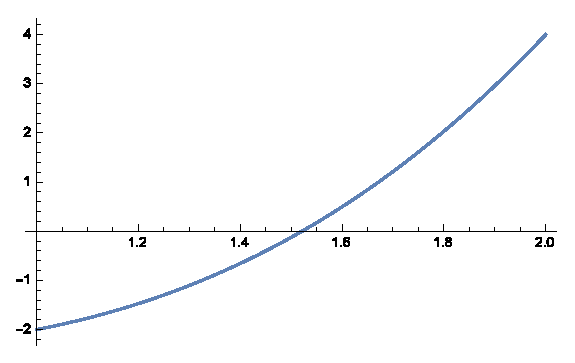
\includegraphics{Graph3}
		\caption{$ f(x) = x^3 - x -2 $}
	\end{figure}
\end{frame}

\begin{frame}[fragile]
	\frametitle{Criterio de terminación y estimados de error:}
	Para este método (preguntar al Profesor o a mi acerca de como elegir este:)
	\[ \epsilon_a = \left| \dfrac{ x_r^{\textrm{nuevo}} - x_r^{\textrm{viejo}} }{x_r^{\textrm{nuevo}}} \right| \cdot 100 \%\]
\end{frame}

\begin{frame}[fragile]
	
\begin{algorithm}[H]
	\begin{algorithmic}[1]
	\REQUIRE $ f,n_{max}, \epsilon,a,b $ 
	\STATE $ n \leftarrow 1 $
	\WHILE{$ n \leq n_{max} $}
		\STATE $ c \leftarrow \frac{a + b}{2} $
		\IF{$ f(c) = 0 $ or $ (b-a)/2 < \epsilon $} 
			\STATE Solución encontrada
			\PRINT c
			\ENDIF
		\STATE{$N \leftarrow N + 1$ } \COMMENT{ Incrementar el contador}
		\IF{$ \operatorname{sign}(f(c)) = \operatorname{sign}(f(a)) \implies a \leftarrow c \textrm{ or } b \leftarrow c  $}
		\STATE{Solucion}
		\ENDIF
		
		
		
	\ENDWHILE
	\end{algorithmic}
	\caption{Pseudocodigo para bisección }
	\label{alg:seq}
\end{algorithm}
\end{frame}

\section{Métodos abiertos}

\begin{frame}[fragile, shrink]
	\frametitle{Métodos abiertos}
	\begin{block}{Métodos abiertos}
		Los métodos abiertos son algoritmos de búsqueda que solo requieren de un solo punto de inicio.
	\end{block}
		\centering
		\adjustbox{max height=\dimexpr\textheight-5.5cm\relax,
			max width=\textwidth}{
			\begin{tabular}{|c|c|c|}
				\hline Metodos & Caracteristica & Función de Iteración \\ 
				\hline Iteracion de punto fijo & secuencia de puntos convergente. & Sea $f(x) $ rescribamos $ x = g(x) $ \\ 
				\hline El metodo de la Secante & Se requieren dos puntos de inicio & $ x_{i+1} = x_i - \frac{f(x_i)(x_{i-1}-x_i)}{f(x_{i-1}) - f(x_i)} $\\ 
				\hline Newton Raphson & El mas usado& $ x_{i+1} = x_i - \frac{f(x_i)}{f'(x_i)} $ \\ 
				\hline Metodo Brent & Combina lo mejor de métodos abiertos y cerrados & Tarea \\ 
				\hline 
			\end{tabular} 
		}
\end{frame}









	
\end{document}